\documentclass[a4paper,12pt]{article}
\setlength{\parindent}{0cm}
\usepackage{amsmath, amssymb, amsthm, mathtools,pgfplots}
\usepackage{graphicx,caption}
\usepackage{verbatim}
\usepackage{venndiagram}
\usepackage[cm]{fullpage}
\usepackage{fancyhdr}
\usepackage{tikz,multirow}
\usepackage{listings}
\usepackage{color,enumerate,framed}
\usepackage{color,hyperref}
\definecolor{darkblue}{rgb}{0.0,0.0,0.5}
\hypersetup{colorlinks,breaklinks,
            linkcolor=darkblue,urlcolor=darkblue,
            anchorcolor=darkblue,citecolor=darkblue}

%\usepackage{tgadventor}
%\usepackage[nohug]{diagrams}
\usepackage[T1]{fontenc}
%\usepackage{helvet}
%\renewcommand{\familydefault}{\sfdefault}
%\usepackage{parskip}
%\usepackage{picins} %for \parpic.
%\newtheorem*{notation}{Notation}
%\newtheorem{example}{Example}[section]
%\newtheorem*{problem}{Problem}
\theoremstyle{definition}
%\newtheorem{theorem}{Theorem}
%\newtheorem*{solution}{Solution}
%\newtheorem*{definition}{Definition}
%\newtheorem{lemma}[theorem]{Lemma}
%\newtheorem{corollary}[theorem]{Corollary}
%\newtheorem{proposition}[theorem]{Proposition}
%\newtheorem*{remark}{Remark}
%\setcounter{section}{1}

\newtheorem{thm}{Theorem}[section]
\newtheorem{lemma}[thm]{Lemma}
\newtheorem{prop}[thm]{Proposition}
\newtheorem{cor}[thm]{Corollary}
%\newtheorem{defn}[thm]{Definition}
\newtheorem*{defn}{Definition}
\newtheorem*{examp}{Example}
\newtheorem{conj}[thm]{Conjecture}
\newtheorem{rmk}[thm]{Remark}
\newtheorem*{nte}{Note}
\newtheorem*{notat}{Notation}
%\pgfplotset{compat=1.14}
%\diagramstyle[labelstyle=\scriptstyle]

\lstset{frame=tb,
  language=Oz,
  aboveskip=3mm,
  belowskip=3mm,
  showstringspaces=false,
  columns=flexible,
  basicstyle={\small\ttfamily},
  breaklines=true,
  breakatwhitespace=true,
  tabsize=3
}

\usepackage{floatrow}
% Table float box with bottom caption, box width adjusted to content
\newfloatcommand{capbtabbox}{table}[][\FBwidth]

\pagestyle{fancy}




\fancyhead{}
\renewcommand{\headrulewidth}{0pt}

\lfoot{}
\cfoot{}

%\lfoot{\color{black!60}{\sffamily Zhangsheng Lai}}
%\cfoot{\color{black!60}{\sffamily Last modified: \today}}
\rfoot{\textsc{\thepage}}



\begin{document}
\flushright{Nguyen Tan Thai Hung\quad 1001986\\Zhangsheng Lai\quad1002554}
\section*{Algorithmic Game Theory: HW 1}

\begin{enumerate}
\item To show the desired inequality, it suffices to show that $f(y,z) = 5y^2+z^2-3zy-3y \geq 0$ for every $y, z \in \{0,1,2,\ldots\}$. We shall use $\mathbb{Z}_{>0}$ to denote the set $\{0,1,2,\ldots\}$ subsequently. We can rewrite $f(y,z)$ to get
\begin{align}
f(y,z) = \left(\frac{3}{2}y-z\right)^2+\frac{11}{4}y^2-3y \label{eq:pos}
\end{align}
which we will show that the $f(y,z)$ in this form is nonnegative. All that is left to show is that  $\frac{11}{4}y^2-3y \geq 0$ for all $y\in \mathbb{Z}_{>0}$ but solving for the inequality, we have
\begin{align*}
\frac{11}{4}y^2-3y \geq 0 \Leftrightarrow y \geq \frac{12}{11} \text{ or } y=0
\end{align*}
meaning we are left to prove that (\ref{eq:pos}) holds for all $z \in \mathbb{Z}_{>0}$ when $y=1$. Solving for the inequality below, 
\begin{align*}
f(1,z)=\left(z-\frac{3}{2}\right)^2-\frac{1}{4} < 0 &\Leftrightarrow (z-1)(z-2)< 0\\
&\Leftrightarrow 1<z<2
\end{align*} 
which says that $f(1,z)<0$ for $z \in (1,2)$ and hence positive for all $z \in \mathbb{Z}_{>0}$ and we are done.

\item 
\begin{enumerate}[(i)]
\item In an nonatomic congestion games with multicommodity networks, let $\mathcal{P}_i$ denote the set of paths from an origin $s_i$ to a sink $t_i$ with $\mathcal{P}_i\neq \emptyset$.
\begin{defn}[flow]
For a \emph{flow} $f$ and path $P \in \mathcal{P}_i$, $f_P$ is the amount of traffic of commodity $i$ that chooses the path $P$ to travel from $s_i$ to $t_i$. A flow is feasible for a vector $r=(r_1,\ldots,r_k)$ if it routes all the traffic: for each $i\in \{1, 2, \ldots, k\}$, $\sum_{P\in \mathcal{P}_i}f_P=r_i$.
\end{defn}
\begin{defn}[Nonatomic equilibrium flow]
Let $f$ be a feasible flow for an nonatomic congestion games with multicommodity networks. The flow $f$ is an \emph{equilibrium flow} if, for every commodity $i \in \{1,2, \ldots, k\}$ and every pair $P, \tilde{P} \in \mathcal{P}_i$ of $s_i-t_i$ paths with $f_P>0$, 
\begin{align*}
c_p(f) \leq c_{\tilde{P}}(f)
\end{align*}
where $c_p(f)$ denotes the cost of travelling on path $P$ for flow $f$.
\end{defn}
\item Let $\mathcal{P}=\bigcup_{i=1}^{k}\mathcal{P}_i$. Then the total cost of a multicommodity network is 
\begin{align*}
\sum_{P\in \mathcal{P}}c_p(f_p)\cdot f_p = \sum_{e\in E}c_e(f_e)\cdot f_e
\end{align*}
where $E$ is the set of directed edges on the graph $G$.

\item
Let $L_i$ be the common cost of all paths in use between $s_i$ and $t_i$ at equilibrium.
\begin{equation}\label{eq:SC_NE}
\text{SC(NE)} = \sum_{i=1}^{k}\sum_{p\in\mathcal{P}_i}f_Pc_P(f) = \sum_{i=1}^{k}r_iL_i 
\end{equation}
On the other hand, for each source-sink pair $s_i-t_i$
\[ \sum_{P\in\mathcal{P}_i}f^*_Pc_P(f)\geq r_iL_i \]
\begin{equation}\label{eq:hybrid}
\Rightarrow \sum_{i=1}^{k}\sum_{P\in\mathcal{P}_i}f^*_Pc_P(f)\geq \sum_{i=1}^{k}r_iL_i
\end{equation}
Now, substract (\ref{eq:SC_NE}) from (\ref{eq:hybrid}) and express the sum as summing over edges instead of over paths, we have
\begin{equation}\label{eq:hybrid2}
\sum_{e\in\mathcal{E}}(f_e^*-f_e)c_e(f_e) \geq 0
\end{equation}
Apply the Pigou bound for each edge with $c\leftarrow c_e, r \leftarrow f_e$ and $x \leftarrow f_e^*$.
\begin{align*}
	\alpha(C) &\geq \frac{rc(r)}{xc(x)+(r-x)c(r)}\\
	\Rightarrow 	\alpha(C) &\geq \frac{f_ec_e(f_e)}{f_e^*c_e(f_e^*)+(f_e-f_e^*)c_e(f_e)}\\
	\sum_{e \in \mathcal{E}}f_e^*c_e(f_e^*) & \geq \sum_{e \in \mathcal{E}} \frac{1}{\alpha(C)}f_ec_e(f_e) + (f_e^* - f_e)c_e(f_e)\\
	\text{SW(OPT)} &\geq \frac{1}{\alpha(C)}\text{SW(NE)}\\
	\alpha(C) &\geq \text{PoA}
\end{align*}

\item We start by showing that 
\begin{align*}
\inf_{x}\left\{\left(\frac{ax+b}{ar+b}-1\right)\right\}&=\inf_{x}\left\{x\left(\frac{a(x-r)}{ar+b}\right)\right\}\\
&=\frac{a}{ar+b}\inf_{x}\left\{x^2-rx\right\}\\
&=-\frac{r^2}{4}\cdot\frac{a}{ar+b}\\
\end{align*}
with that we can begin out proof.
\begin{align*}
\sup_{c\in \mathcal{C}}\sup_{x,r}\frac{rc(r)}{x c(x)-(r-x)c(r)}&=\sup_{c\in \mathcal{C}}\sup_{x,r}\frac{r}{r +x\left(\frac{c(x)}{c(r)}-1\right)}, \text{ since $c(r)>0$}
\\
&=\sup_{a,b\geq0}\sup_{x,r}\frac{r}{r +x\left(\frac{ax+b}{ar+b}-1\right)}\\
&=\sup_{a,b\geq0}\sup_{r}\frac{r}{r -\frac{r^2}{4}\frac{a}{ar+b}}\\
&=\sup_{a,b\geq0}\sup_{r}\frac{1}{1 -\frac{ar}{4(ar+b)}}\\
&=\frac{1}{1-1/4}
\end{align*}
the last equality follows as the supremum of $\frac{ar}{4(ar+b)}$ occurs when $b=0$.
\end{enumerate}

\item
\begin{enumerate}[(i)]
\item Let $\Phi$ be the potential function of a potential game and $c_i$ denote the cost function of the agents for $i\in \{1,2,\ldots,k\}$. 
%If $s=(s_1,\ldots,s_{i-1},s_i,s_{i+1},\ldots,s_k)$ and $s'_i \neq s_i$ is any alternative strategy for agent $i$ for $i\in \{1,2,\ldots,k\}$, we have
%\begin{align*}
%c_i(s_i,s_{-i})-c_i(s'_i,s_{-i})=\Phi(s_i,s_{-i})-\Phi(s'_i,s_{-i})
%\end{align*}
To prove the required, it suffices to show that 
\begin{align*}
c_i(s_i,s_{-i})-\Phi(s_i,s_{-i})
\end{align*}
is independent of the choice of $s_i$ and solely dependent on $s_{-i}$. If we consider two alternative distinct strategies for agent $i$, $s'_i, s''_i \neq s_i$
\begin{align*}
c_i(s_i,s_{-i})&=\Phi(s_i,s_{-i})+\left[c_i(s'_i,s_{-i})-\Phi(s'_i,s_{-i})\right]\\
c_i(s_i,s_{-i})&=\Phi(s_i,s_{-i})+\left[c_i(s''_i,s_{-i})-\Phi(s''_i,s_{-i})\right]
\end{align*} 
hence we can choose $D_i(s_{-i})=c_i(-,s_{-i})-\Phi(-,s_{-i})$, where $-$ represents any choice of strategy of agent $i$.

\item Let $\Phi_1$ and $\Phi_2$ be two potential functions of a game. From 3\,(i) we have
\begin{align}
c_i(s_i,s_{-i})&=\Phi_1(s_i,s_{-i})+D^1_i(s_{-i})\label{eq:3ii1}\\
c_i(s_i,s_{-i})&=\Phi_2(s_i,s_{-i})+D^2_i(s_{-i})\label{eq:3ii2}
\end{align}
where $D^k_i(s_{-i})$ denotes the dummy term for $k=1,2$. Taking (\ref{eq:3ii1})$-$(\ref{eq:3ii2}), 
 \begin{align*}
\Phi_1(s_i,s_{-i})-\Phi_2(s_i,s_{-i})=D^1_i(s_{-i})-D^2_i(s_{-i})
\end{align*}
we have shown that two distinct potential functions differ by a constant, more precisely the difference of their dummy term evaluated at $s_{-i}$ and any strategy of agent $i$, $s_i$.

\item
First, we prove that for any potential game, the equality holds. Let $\Phi$ be a potential function. By definition,
\[ c_i(s^2_i, s^1_{-i}) - c_i(s^1) = \phi(s^2_i,s^1_{-i}) - \phi(s^1)\]
Furthermore, from part (i) we have
\[ c_i(s^2) = \phi(s^2) + D_i(s^2_{-i}) \]
and the same results apply for agent $j$. So
\begin{align*}
\text{LHS} &= c_i(s^2_i,s^1_{-i})-c_i(s^1)+c_j(s^2)-c_j(s^2_i,s^1_{-i})\\
&=\phi(s^2_i,s^1_{-i})-\phi(s^1) -c_j(s^2_i,s^1_{-i}) + \phi(s^2)+D_j(s^2_{-j}) \\
&= \phi(s^2)-\phi(s^1) + D_j(s^2_{-j}) - D_j(s^2_i, s^1_{-i})
\end{align*}
Now, observe that $D_j(s^2_{-j})=D_j(s^2_i, s^1_{-i})$ because in both cases $i$ plays $s_i^2$ while the rest of the players (different from $i$ and $j$) play the same in $s^1$ and $s^2$ anyways. Therefore
\[ \text{LHS}= \phi(s^2)-\phi(s^1)\]
In the same manner we prove that RHS = $\phi(s^2)-\phi(s^1)$. Therefore, for any potential game, LHS = RHS.

Now we need to prove the reverse, i.e. if the identity holds for every pair $s^1, s^2$ then the potential function exists. We want to show that for every pair $i,j$, 
\[c_i(s^2_i, s^1_{-i}) - c_i(s^1) = \phi(s^2_i, s^1_{-i}) - \phi(s^1)\] 
and so on. Our idea is to use the observation that $(s^2_i, s^1_{-i})$ and $(s^1_j, s^2_{-j})$ are the same outcome, and manipulate terms so that the relationship $D_j(s^2_{-j})=D_j(s^2_i, s^1_{-i})$ appears, which links us back to the first part.
\end{enumerate}

\item
\begin{enumerate}[(a)]
\item Let $\tilde{f}$ be an equilibrium flow for an atomic selfish routing network of parallel links. Then for every player $i \in \{1,2,\ldots, n\}$, any two parallel links $P_i,P_j$ where $1\leq i < j \leq k$,
\begin{align*}
c_{P_i}(\tilde{f})\leq c_{P_j}(f)
\end{align*}
here, the flow of $\tilde{f}$ on $P_i$ equals the flow of $f$ on $P_j$, $(\tilde{f}_{P_i}=f_{P_j})$ i.e. any player routing their commodity to any path will have a cost equal to or larger than the equilibrium flow.
\begin{align*}
\sum_{m=1}^{\tilde{f}_{P_i}}c_{P_i}(m)\leq \sum_{m=1}^{f_{P_j}}c_{P_j}(m)
\end{align*}
since the above inequality is true for any two parallel links, we sum it over the $n$ parallel links and we are done.
\begin{align*}
\Phi(\tilde{f})=\sum_{i=1}^{n}\sum_{m=1}^{\tilde{f}_{P_i}}c_{P_i}(m)\leq \sum_{i=1}^{n}\sum_{m=1}^{f_{P_i}}c_{P_j}(m)=\Phi(f)
\end{align*}
where $\Phi$ is the potential function.

\item
Consider the triangular network of internet service providers (ISP) that we discussed in class (Figure \ref{fig:3gon}). There are 3 ISPs 1, 2, 3 serving a common market located at 4. Suppose the direct links from the ISPs to the user has high cost, and the links between the ISPs are cheap. Now, if 1 is using the direct link 1-4, then 3 will have an incentive to piggy-back ride and use 3-1-4, abandoning the link 3-4. Then 2 has two choices: either to use his own direct link 2-4, or to use a 3-hop link 2-3-1-4. The latter is not desirable (as it will cause a lot of delay), so he will bear the high cost and run the link 2-4. When that's the case, 1 will have the incentive to piggy-back ride, abandoning 1-4 and using 1-2-4 instead. But this will cause 3 to choose the direct link 3-4 instead of piggy-back ride through 1. This is contrary to his previous strategy. The cycle repeats. Effectively, there are no Nash equilibria in this game.

\newdimen\R
\R=2cm
\begin{figure}[h]
	\centering
	\begin{tikzpicture}[scale=1.5]
	\tikzstyle{neuron}=[circle,fill=black!25,minimum size=15pt,inner sep=0pt]
	\tikzstyle{m}=[neuron, fill=red!50];
	\tikzstyle{n}=[neuron, fill=blue!50];
	
	\draw[rotate=90,color=white] (0:\R) \foreach \x in {1,2,3} {
		node[n](\x){\color{white}{\x}} -- (\x*120:\R) 
	};%-- (90:\R) ;%node[above] {t} ;%cycle (90:\R) node[above] {t} ;
	%\node[xshift=-6cm,below=2pt] at (-36:2.25){\footnotesize $a_{i-1}$};
	%\node[xshift=-6cm,below=2pt] at (-30:3.5){\footnotesize $a_i$};
	%\node[xshift=-6cm,below=2pt] at (-18:4.5){\footnotesize $a_{i+1}$}; 
	\node[n](c) at (0:0){\color{white}{4}}; 
	\draw[->,thick] (1) -- (c); 
	\draw[->,thick] (3) -- (c); 
	\draw[->,thick] (2) -- (c); 
	\draw[->,thick] (1) -- (2);
	\draw[->,thick] (2) -- (3);
	\draw[->,thick] (3) -- (1);
	% \draw[xshift=3cm] (-144:\R) \foreach \x in {-108,-72,...,215} {
	% node[m]{} -- (\x:\R) 
	% };
	%\node[below=2pt] at (-36:2.25){\footnotesize $b_{i-1}$};
	%\node[below=2pt] at (-30:3.5){\footnotesize $b_i$};
	%\node[below=2pt] at (-18:4.5){\footnotesize $b_{i+1}$};
	% \draw[xshift=3cm] (0:\R) \foreach \x in {36,72,...,359} {
	% node[m]{} -- (\x:\R) 
	% } -- cycle (90:\R) node[above] {} ;
	\end{tikzpicture}
	\caption{Example network with non-parallel links}
	\label{fig:3gon}
\end{figure}

\end{enumerate}

\item
\begin{enumerate}[(a)]
\item %The approach to find construct the bijection from the strategies from a partnership game $G^1$ to a congestion game $G^2$ will be to first find one for a 2 player game where the player have $2$ strategies respectively. 
The congestion game to consider is shown below with $m=n=2$  where $n$ and $m$ are the number of strategies for P1 and P2 respectively,. A strategy of P1 is the upper or lower edges of the networks; we shall let $A_1$ be the upper edges. A strategy of P2  is the choice of a disjoint network, here the left network is P2's strategy $B_1$. For  $1\leq i \leq n$ and  $1\leq j \leq m$, $e_{i,j}$ is the $i$th edge of the $j$th disjoint network.

\begin{figure}[h]
\begin{floatrow}
\ffigbox{%
\def\layersep{1.5cm}

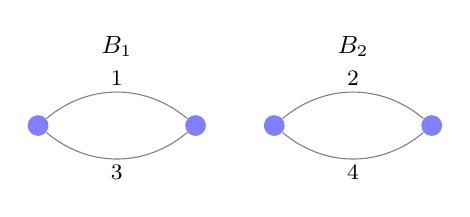
\begin{tikzpicture}[scale = 1,
%shorten >=1pt,->,
draw=black!50, node distance=\layersep]
    %\tikzstyle{every pin edge}=[<-,shorten <=1pt]
    \tikzstyle{neuron}=[circle,fill=black!25,minimum size=7.5pt,inner sep=0pt]
    \tikzstyle{output neuron}=[neuron, fill=red!50];
    \tikzstyle{n}=[neuron, fill=blue!50];

\node[n] (a) at (0,0) {};
\node[n] (b) at (2,0) {};
\node[n] (c) at (3,0) {};
\node[n] (d) at (5,0) {};
%\node[n] (e) at (6,0) {};
%\node[n] (f) at (8,0) {};
%\node at (5.5,0) {$\ldots$};
\node at (1,1) {\small $B_1$};
\node at (4,1) {\small $B_2$};
\foreach \y in {-40,40}{
%\foreach \y in {-40,0,40}{
%\draw (a) edge[bend right] node[below] {\small $2$} (b);
%\draw (a) edge[bend left] node[above] {\small $x$} (b);
\draw  (a) edge[bend left=\y] node[above] {} (b);
\draw (c) edge[bend left=\y] node[above] {} (d);
%\draw (e) edge[bend left=\y] node[above] {} (f);
};
\node at (1,0.6) {\footnotesize 1};
\node at (1,-0.6) {\footnotesize 3};
\node at (4,0.6) {\footnotesize 2};
\node at (4,-0.6) {\footnotesize 4};
\end{tikzpicture}
%
}{%
% \caption{A network for a $2 \times 2$ partnership game.}%
}
\capbtabbox{%
\footnotesize
\renewcommand{\arraystretch}{1.5}
    \centering
    \begin{tabular}{cc|c|c|}
      & \multicolumn{1}{c}{} & \multicolumn{2}{c}{P$2$}\\
      & \multicolumn{1}{c}{} & \multicolumn{1}{c}{$B_1$}  & \multicolumn{1}{c}{$B_2$} \\\cline{3-4}
      \multirow{2}*{P$1$}  & $A_1$ & $1,1$ & $2,2$ \\\cline{3-4}
      & $A_2$ & $3,3$ & $4,4$ \\\cline{3-4}
    \end{tabular}
}{%
 % \caption{\footnotesize A $2\times 2$ partnership game}%
}
\end{floatrow}
%\caption{A congestion network corresponding to a partnership game.}
\end{figure}

%We shall denote an edge in the network as $e_{ij}$, where $1\leq i \leq n$ is the edge chosen in a network and $1 \leq j\leq m$ where $n$ and $m$ are the number of strategies for P1 and P2 respectively is a chosen network.
Hence the tuple of bijective functions from the strategies of the network to the strategies in the partnership game for the congestion game shown above is:
\begin{alignat*}{4}
f_1(A_i,B_j)&=\{e_{i,j}\}_{1\leq j\leq m}, &\quad&\text{the $i$th edge in every disjoint network }\\
f_2(A_i,B_j)&=\{e_{i,j}\}_{1\leq i\leq n}, &\quad &\text{all the edges in the $j$th disjoint network}\\
\end{alignat*}
which says that every strategy in the congestion game is a subset of edges in the family of disjoint networks. The cost function $c^1_k$ for the partnership game $G^1$ is shown in the table above and the cost function for the congestion game $c_k^2(\{e_{p,j}\}_{1\leq j \leq m},\{e_{i,q}\}_{1\leq i \leq n})$ is the cost of the unique edge found from the intersection $\{e_{p,j}\}_{1\leq j \leq m}\cap\{e_{i,q}\}_{1\leq i \leq n}$. Note that although we used fixed numbers as the cost in the 2 player 2 strategies example we illustrated above, we can see them as just placeholders and it works well for any partnership game of that form even with different cost. We can generalize this from 2 players to $N$ players in a similar fashion.

 
%\begin{figure}
%\centering
%\def\layersep{1.5cm}
%
%\begin{tikzpicture}[scale = 1,shorten >=1pt,->,draw=black!50, node distance=\layersep]
%    \tikzstyle{every pin edge}=[<-,shorten <=1pt]
%    \tikzstyle{neuron}=[circle,fill=black!25,minimum size=7.5pt,inner sep=0pt]
%    \tikzstyle{output neuron}=[neuron, fill=red!50];
%    \tikzstyle{n}=[neuron, fill=blue!50];
%
%\node[n] (a) at (0,0) {};
%\node[n] (b) at (2,0) {};
%\node[n] (c) at (3,0) {};
%\node[n] (d) at (5,0) {};
%\node[n] (e) at (6,0) {};
%\node[n] (f) at (8,0) {};
%\node at (5.5,0) {$\ldots$};
%\foreach \y in {-40,-20,0,20,40}{
%\foreach \y in {-40,0,40}{
%\draw (a) edge[bend right] node[below] {\small $2$} (b);
%\draw (a) edge[bend left] node[above] {\small $x$} (b);
%\draw  (a) edge[bend left=\y] node[above] {} (b);
%\draw (c) edge[bend left=\y] node[above] {} (d);
%\draw (e) edge[bend left=\y] node[above] {} (f);
%};
%\end{tikzpicture}
%\caption{A two player game with where each player has $n,m$ strategies respectively. }
%\end{figure}

\item 
Still working on it.
\item We know that the cost function of a potential game can be decomposed into the sum of a potential function and a dummy function. We claim that:
\begin{enumerate}
\item in a partnership game, the potential function is $\phi(s)=c_i(s) \; \forall i$. Therefore, the cost function of a partnership game which is also a potential game, can be decomposed into a sum of a potential function and a zero function as its dummy function 
\[ c_i(s) = \phi(s) + \mathbf{0}\]
\item in a dummy game, the potential function is $\phi(s) = 0$. The cost function of a dummy game which is also a potential game can be decomposed into a sum of itself as the dummy function and a potential function which is the zero function.
\[ c_i(s) = \mathbf{0} + D_i(s_{-i})\]
\end{enumerate}
Now, if we have a potential game such that
\[ c_i(s) = \phi(s) + D_i(s_{-i})\]
then we can effectively map the partnership game with potential function $\phi(s)$ into a congestion game $G_1$ and map the dummy game with dummy function $D_i(s_{-i})$ into another congestion game $G_2$. What we did is effectively map a potential game into a congestion game with two separate networks $G_1$ and $G_2$, where each player has to play an action in $G_1$ and an action in $G_2$ simultaneously (isomorphism is preserved under addition). Thus every potential game is isomorphic to a congestion game.


%Let $P$ and $D$ denote a partnership and dummy game respectively that $C^1, C^2$ be the respective congestion game they are isomorphic to. Then $P\times D$ is isomorphic to $C^1\times C^2$. Since the cartesian product of congestion games is also a congestion game, we have that the cartesian product of a partnership and dummy game isomorphic to a congestion game. Since a partnership game is a potential game, it suffices to show that 
%
%
%a dummy game is a potential game. 
%\begin{align*}
%%\Phi(s_i,s_{-i})-\Phi(s^\ast_i,s_{-i})=
%c_i(s_i,s_{-i})-c_i(s^\ast_i,s_{-i})=D_i(s_{-i})-D_i(s_{-i})=0
%\end{align*}
%we can choose the potential function $\Phi(s)$ to be the zero function thus it is shown that dummy games are potential games. Now,

\end{enumerate}


\item
\begin{enumerate}[(a)]
\item We consider two networks $A, B$ that resemble $n-$gons where $n$ is even, i.e. there are $n$ edges and $n$ vertices for each network as shown in Figure \ref{fig:ngon}. The strategy of each player $i$ is 
\begin{align*}
S_i=\{\{a_i,b_i\},\{a_{i+1},b_{i-1},b_{i+1}\}\}=\{s_i^1,s_i^2\}
\end{align*}
where $a_i,b_i$ denotes edges in $A$ and $B$ respectively and the cost function of each edge is simply $c_e(x)=x$. We claim that when all the player were to play $s_i^1$ it is a Nash equilibrium and we have the optimal value of potential which has value $2n$, since every edge is inhabit by a single player. Any player $i$ that deviates from playing $s_i^1$ will increase the potential by $2+2+2-1$ (hence the claim it is a Nash) since it will share an edge with player $i+1$ in $A$ and players $i-1, i+1$ in $B$ and hence increase the potential. If all the players were to play $s_i^2$, we see that the potential will be $n+n+2n$ where the first $n$ is incurred from $A$ and the next two terms are from $B$ as we sum up the cost from 1 to the load of the edge. It is easy to see that everyone playing $s_i^2$ is a Nash; for any player that deviates from $s_i^2$, will have an increased cost of $+1$ coming from $A$, an increased cost of $+2$ from $B$ and hence this completes the proof. 



\newdimen\R
\R=2cm
\begin{figure}[h]
\centering
\begin{tikzpicture}
\tikzstyle{neuron}=[circle,fill=black!25,minimum size=5pt,inner sep=0pt]
    \tikzstyle{m}=[neuron, fill=red!50];
    \tikzstyle{n}=[neuron, fill=blue!50];

 \draw[xshift=-3cm] (-144:\R) \foreach \x in {-108,-72,...,215} {
              node[n]{}  -- (\x:\R)   
            };%--  (90:\R) ;%node[above] {t} ;%cycle (90:\R) node[above] {t} ;
\node[xshift=-6cm,below=2pt] at (-36:2.25){\footnotesize $a_{i-1}$};
\node[xshift=-6cm,below=2pt] at (-30:3.5){\footnotesize $a_i$};
\node[xshift=-6cm,below=2pt] at (-18:4.5){\footnotesize $a_{i+1}$};            
            
 \draw[xshift=3cm] (-144:\R) \foreach \x in {-108,-72,...,215} {
              node[m]{}  -- (\x:\R)   
            };
\node[below=2pt] at (-36:2.25){\footnotesize $b_{i-1}$};
\node[below=2pt] at (-30:3.5){\footnotesize $b_i$};
\node[below=2pt] at (-18:4.5){\footnotesize $b_{i+1}$};
%             \draw[xshift=3cm] (0:\R) \foreach \x in {36,72,...,359} {
%              node[m]{}  -- (\x:\R) 
%            } -- cycle (90:\R) node[above] {} ;
\end{tikzpicture}
\caption{Example with price of potential anarchy equals 2.}\label{fig:ngon}
\end{figure}

\item
First, we understand that this question is concerning the atomic case, because for the non-atomic case, all Nash equilibria have the same potential value, as we proved in class.
The first obvious bound is that
\begin{align*}
	\phi(s) &\leq SW(s)\\
	\phi(s^*) &\leq SW(s^*)\\
	\Rightarrow PoPA = \frac{\phi(s)}{\phi(s^*)} &\leq PoA = \frac{SW(s)}{SW(s^*)} \leq \frac{5}{2}
\end{align*}
Idea for proving a tight bound: apply the same 4-step strategy as for a normal PoA bound, but the tricky part is that the potential function is not a sum over all agents like the social welfare. Below are what we have got so far:
\[ \phi(s) = \sum_{e\in\mathcal{E}}\sum_{i=1}^{l_e}c_e(i) \]
\[ \phi(s^*) = \sum_{e\in\mathcal{E}}\sum_{i=1}^{l^*_e}c_e(i) \]
Now we create a hybrid term
\begin{align*}
	\phi(s^*_i,s_{-i}) - \phi(s) = \sum_{e\in s^*_i \setminus s_i} c_e(f_e+1) - \sum_{e\in s_i \setminus s^*_i}c_e(f_e) \geq 0
\end{align*}
To go from $\phi(s)$ to $\phi(s^*)$ we let agents deviate one by one
\begin{align*}
	\phi(s) &\leq \phi(s^*_1,s_{-1}) + \sum_{e\in s_1 \setminus s^*_1}c_e(f_e) - \sum_{e\in s^*_1 \setminus s_1} c_e(f_e+1)\\
	&\leq \phi(s^*_1,s^*_2,s_{3..n}) + \sum_{e\in s_1 \setminus s^*_1}c_e(f_e) - \sum_{e\in s^*_1 \setminus s_1} c_e(f_e+1) + \sum_{e\in s_2 \setminus s^*_2}c_e(f_e) - \sum_{e\in s^*_2 \setminus s_2} c_e(f_e+1)\\	\\
	&\leq ...\\
	&\leq \phi(s^*) + \sum_{i=1}^{n} \sum_{e\in s_i \setminus s^*_i}c_e(f_e) - \sum_{i=1}^{n}\sum_{e\in s^*_i \setminus s_i} c_e(f_e+1)
\end{align*}
Now if we can manipulate the double sums so that we can create $\phi(s)$ and $\phi(s^*)$ then we are done. We are trying to break the $c_e(f_e)$ term into two components, one involves $\phi(s)$ and one involves a dummy term.



%\newdimen\R
%\R=2cm
%\begin{figure}[h]
%\centering
%\begin{tikzpicture}[scale=1.5]
%\tikzstyle{neuron}=[circle,fill=black!25,minimum size=15pt,inner sep=0pt]
%    \tikzstyle{m}=[neuron, fill=red!50];
%    \tikzstyle{n}=[neuron, fill=blue!50];
%
% \draw[rotate=90,color=white] (0:\R) \foreach \x in {1,2,3} {
%              node[n](\x){\color{white}{\x}}  -- (\x*120:\R)   
%            };%--  (90:\R) ;%node[above] {t} ;%cycle (90:\R) node[above] {t} ;
%%\node[xshift=-6cm,below=2pt] at (-36:2.25){\footnotesize $a_{i-1}$};
%%\node[xshift=-6cm,below=2pt] at (-30:3.5){\footnotesize $a_i$};
%%\node[xshift=-6cm,below=2pt] at (-18:4.5){\footnotesize $a_{i+1}$};            
%\node[n](c) at (0:0){\color{white}{4}};   
%\draw[->,thick]  (1) -- (c);       
%\draw[->,thick]  (3) -- (c);       
%\draw[->,thick]  (2) -- (c);       
%\draw[->,thick] (1) -- (2);
%\draw[->,thick] (2) -- (3);
%\draw[->,thick] (3) -- (1);
%% \draw[xshift=3cm] (-144:\R) \foreach \x in {-108,-72,...,215} {
%%              node[m]{}  -- (\x:\R)   
%%            };
%%\node[below=2pt] at (-36:2.25){\footnotesize $b_{i-1}$};
%%\node[below=2pt] at (-30:3.5){\footnotesize $b_i$};
%%\node[below=2pt] at (-18:4.5){\footnotesize $b_{i+1}$};
%%             \draw[xshift=3cm] (0:\R) \foreach \x in {36,72,...,359} {
%%              node[m]{}  -- (\x:\R) 
%%            } -- cycle (90:\R) node[above] {} ;
%\end{tikzpicture}
%\caption{Example with price of potential anarchy equals 2.}\label{fig:3gon}
%\end{figure}



 
\end{enumerate}

\end{enumerate}











\end{document}